\documentclass{beamer}
\usepackage{graphics}
\title{Structure and organization of generated hardware}
\author{Madhav P. Desai\\Department of Electrical Engineering\\IIT Bombay, Mumbai, India}
\date{March 8, 2018}
\begin{document}
\maketitle

\frame[containsverbatim]{\frametitle{Top-level view}
\begin{figure}
  \centering
  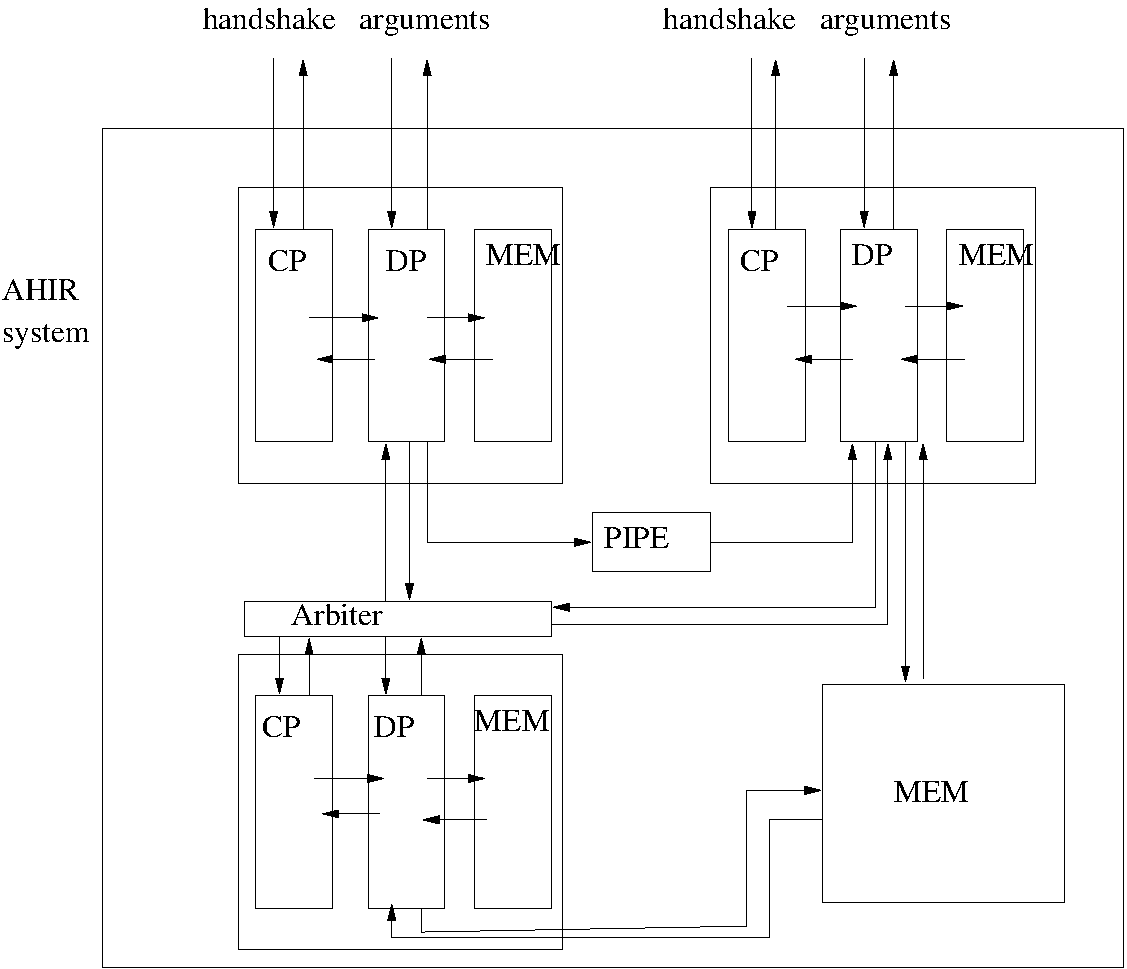
\includegraphics[width=9cm]{figs/TopLevel.pdf}
  \caption{Structure of AHIR system}
\end{figure}
}

\frame[containsverbatim]{\frametitle{The Data-path: a graph of operators and wires}
\begin{figure}
  \centering
  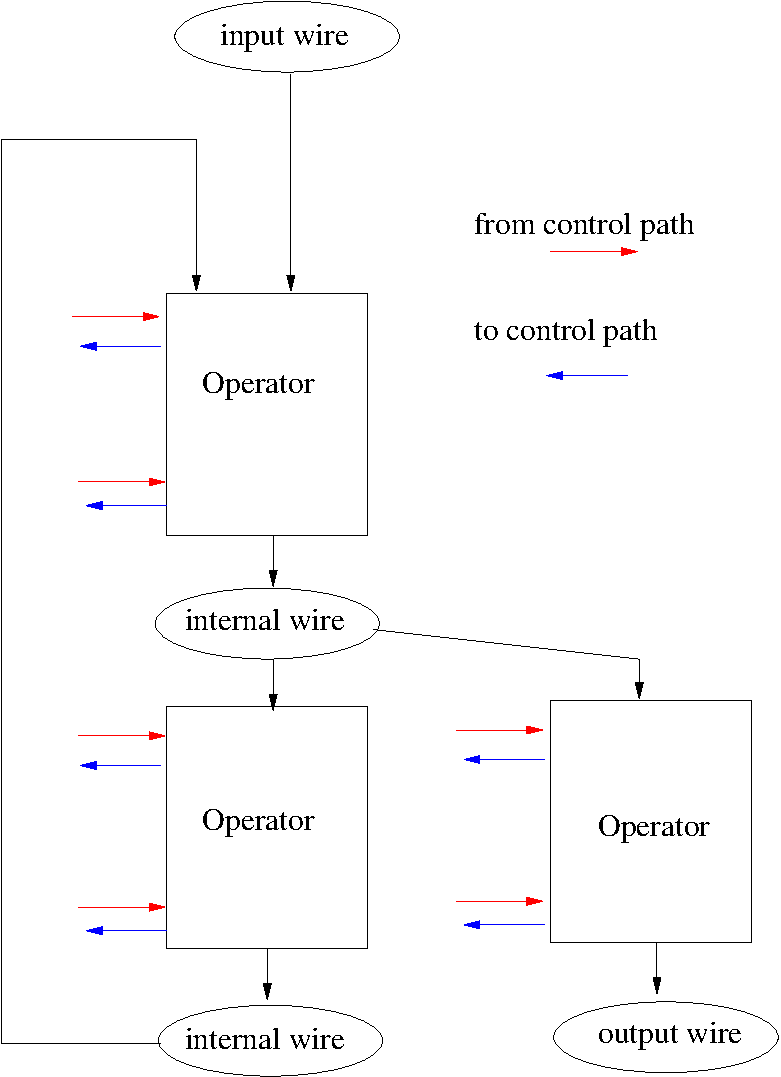
\includegraphics[width=6cm]{figs/DataPath.pdf}
  \caption{Data-path in module of AHIR system}
\end{figure}
}

\frame[containsverbatim]{\frametitle{A generic operator in the data-path}
\begin{figure}
  \centering
  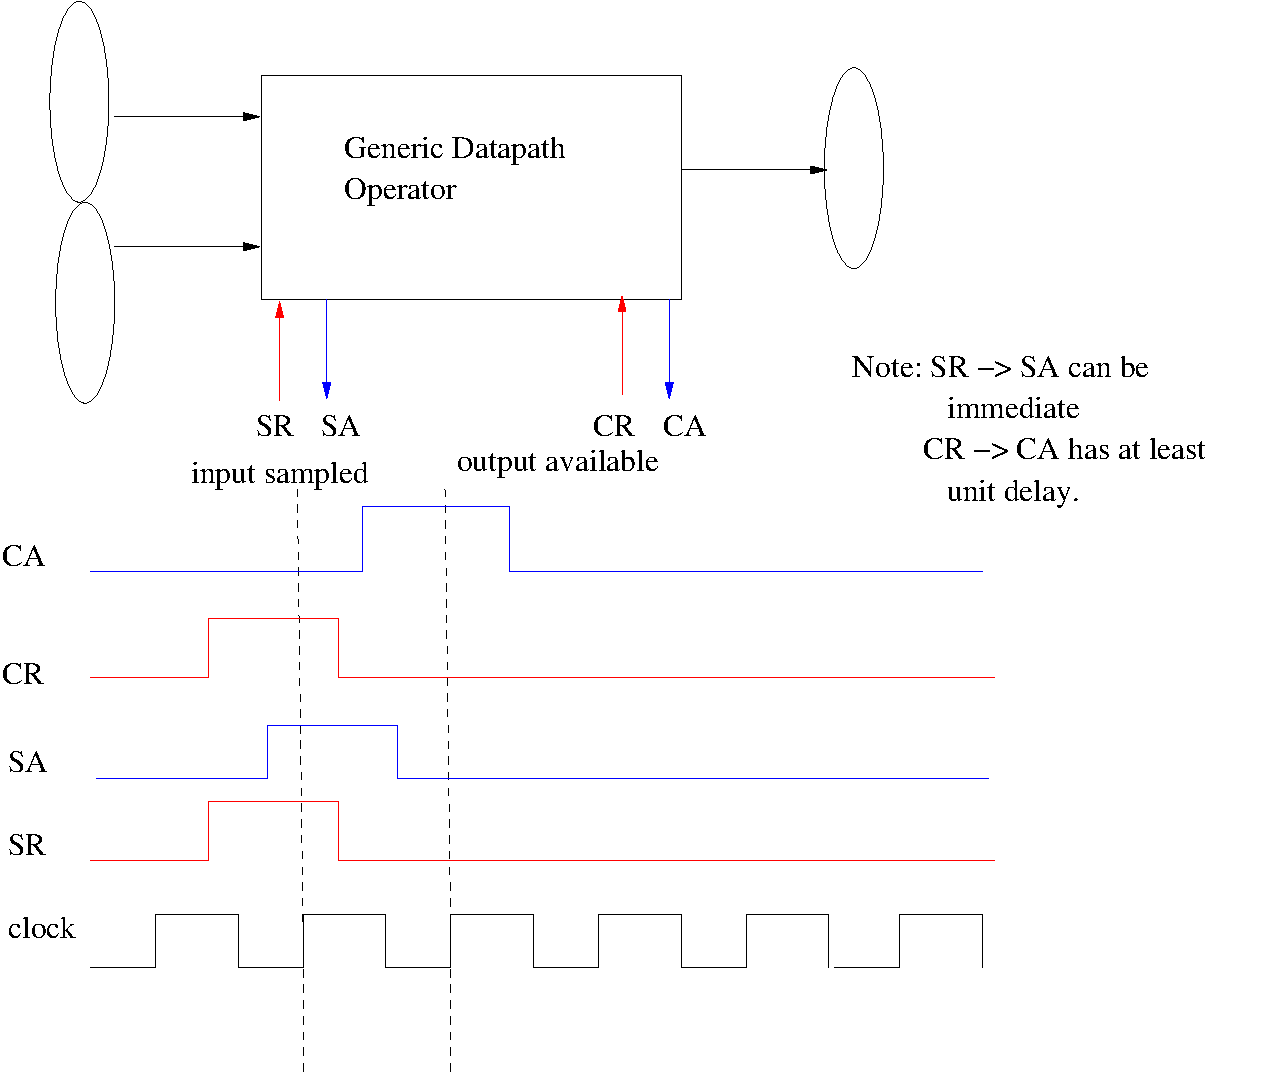
\includegraphics[width=8cm]{figs/GenericOperator.pdf}
  \caption{Generic operator in the data-path}
\end{figure}
}

\frame[containsverbatim]{\frametitle{Operator classes in the data-path}
\begin{itemize}
\item Pure operators: arithmetic, logic.
\item I/O port operators:  input and output ports.
\item Load/Store operators.
\item Shared Call/Return operators:  call-start and call-complete operators.
\item Function operators.
\item Branch operators.
\end{itemize}
}

\frame[containsverbatim]{\frametitle{Input/Output operators in the data-path}
\begin{figure}
  \centering
  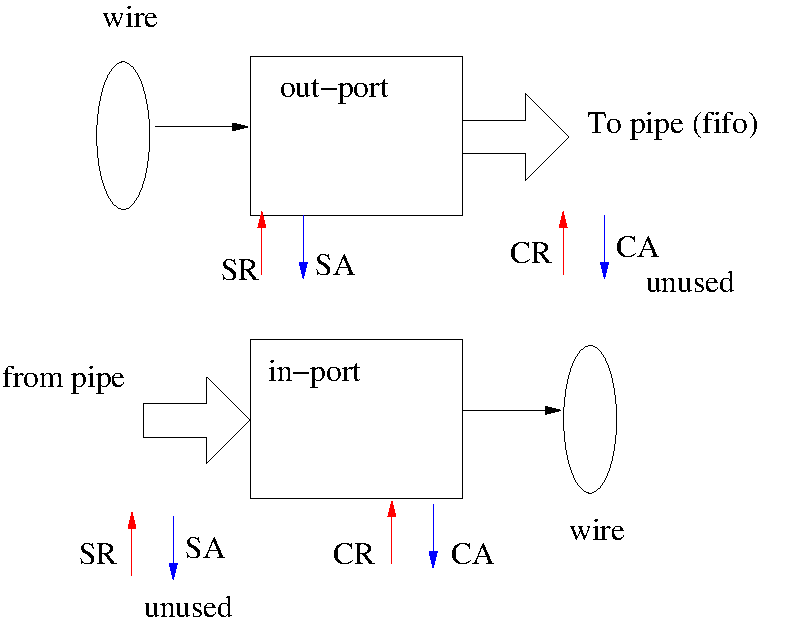
\includegraphics[width=8cm]{figs/IOPorts.pdf}
  \caption{Input/output port operators in the data-path}
\end{figure}
}

\frame[containsverbatim]{\frametitle{Load/Store operators in the data-path}
\begin{figure}
  \centering
  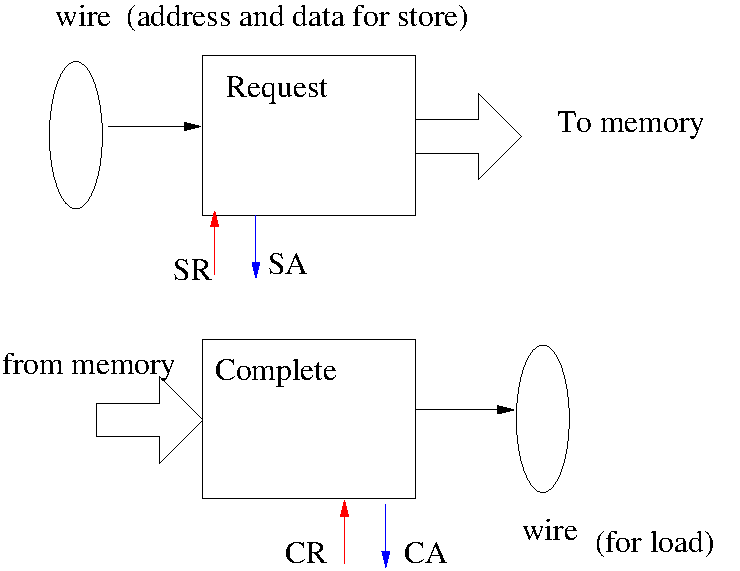
\includegraphics[width=8cm]{figs/LoadStore.pdf}
  \caption{Load/Store operators in the data-path}
\end{figure}
}

\frame[containsverbatim]{\frametitle{Call/Return operators in the data-path}
\begin{figure}
  \centering
  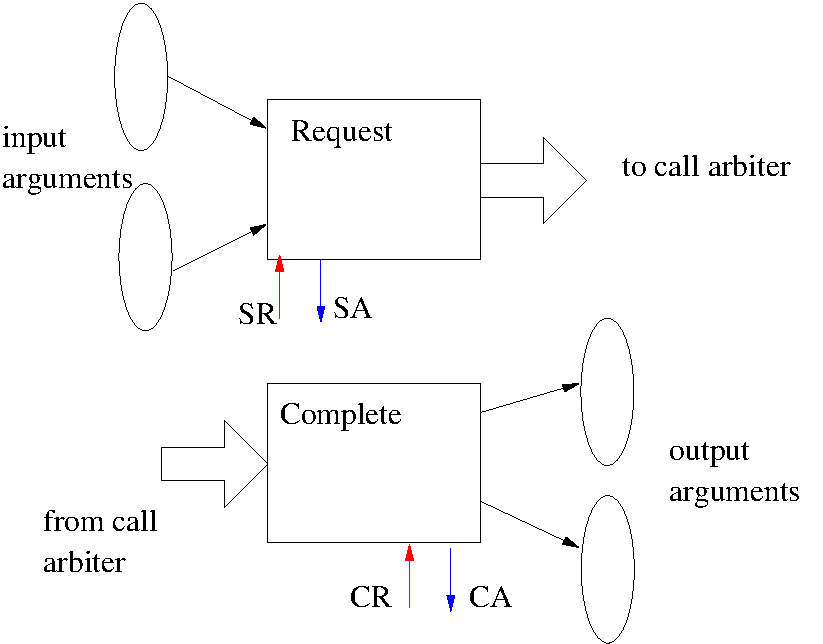
\includegraphics[width=10cm]{figs/CallReturn.pdf}
  \caption{Call/Return operators in the data-path}
\end{figure}
}

\frame[containsverbatim]{\frametitle{Function operators in the data-path}
\begin{figure}
  \centering
  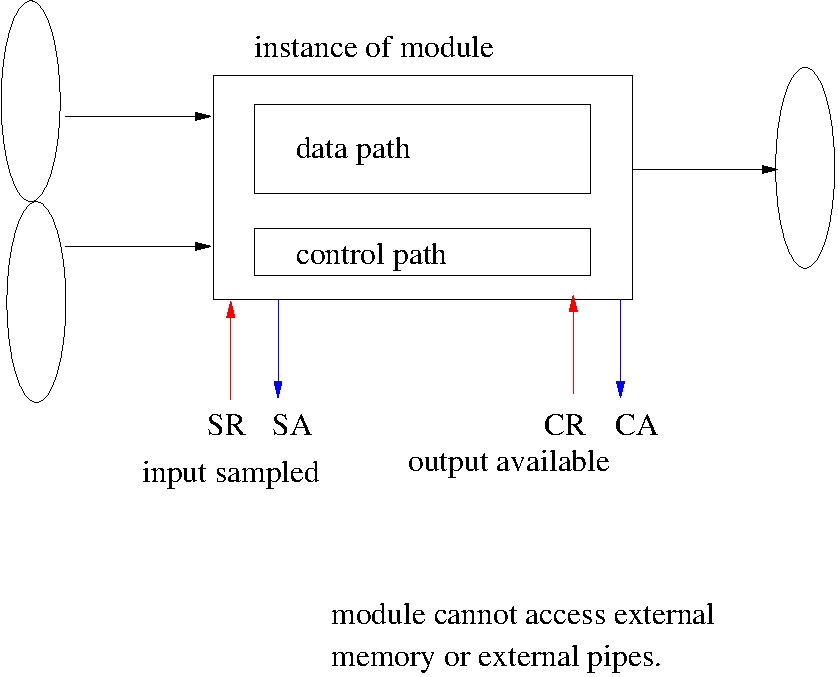
\includegraphics[width=8cm]{figs/Operator.pdf}
  \caption{Function operators in the data-path}
\end{figure}
}

\frame[containsverbatim]{\frametitle{Branch operators in the data-path}
\begin{figure}
  \centering
  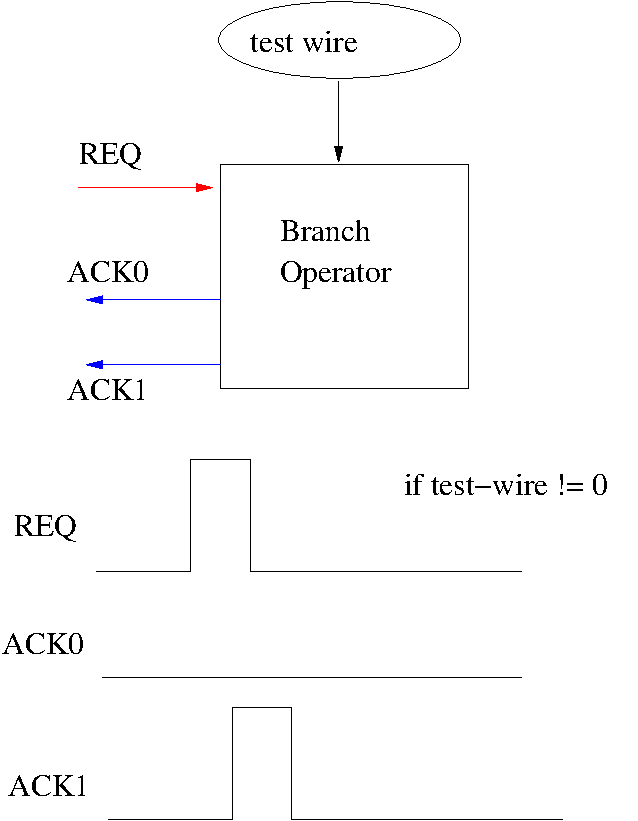
\includegraphics[width=6cm]{figs/BranchOperator.pdf}
  \caption{Branch operators in the data-path}
\end{figure}
}

\frame[containsverbatim]{\frametitle{Data-path: summary}
\begin{itemize}
\item  A  network of wires and data-path operators.
\item  The outputs of data-path operators are registered (buffered).
\item  The amount of buffering at the inputs and outputs can be controlled.
\item  Operators are triggered by control pulses and indicate completion by
status pulses.
\item  A split protocol is followed in all operators.
\end{itemize}
}

\frame[containsverbatim]{\frametitle{The Control-path: a safe Petri-net}
\begin{itemize}
\item A Petri-net is a directed graph with two kinds of vertices
\begin{itemize}
\item Places, which can be thought of as containers which can hold a token.
\item Transitions, which can be thought of as events.
\end{itemize}
\item There are arcs from places to transitions and from transitions to places.
\item A transition is enabled when all its input places have a token.
\item An enabled transition can fire, and firing of a token removes a token
from all input places and puts a token into all output places.
\item The net is safe if it is impossible for a place to ever have more than
one token.
\end{itemize}
}

\frame[containsverbatim]{\frametitle{Examples of Petri-nets}
\begin{figure}
  \centering
  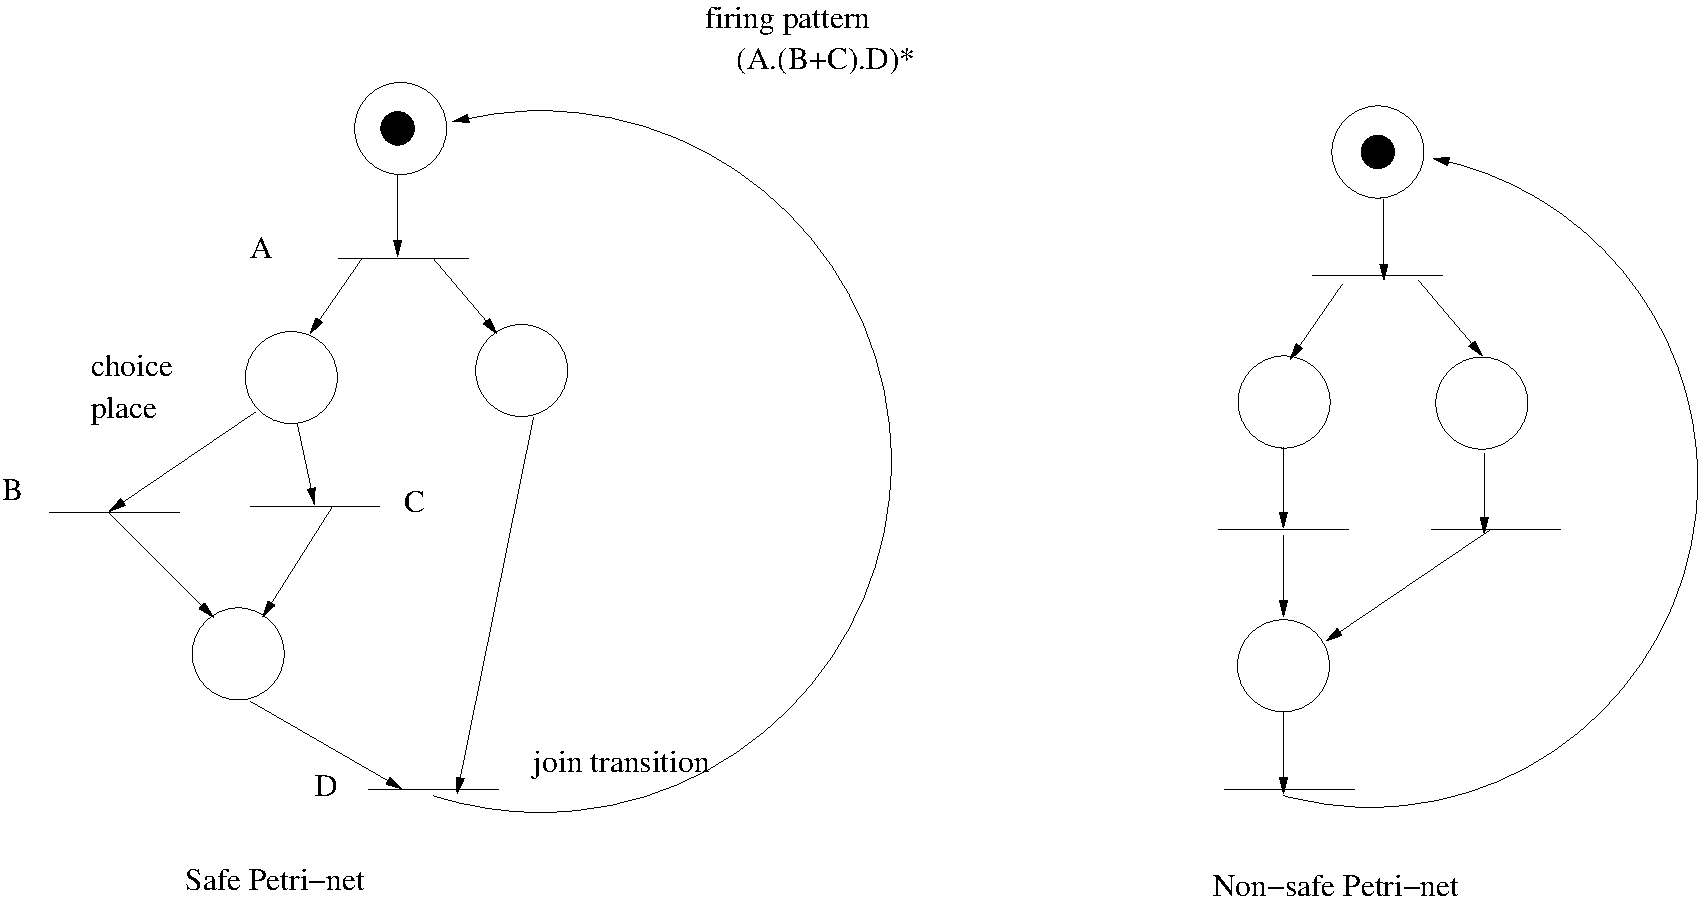
\includegraphics[width=9cm]{figs/ExamplePetriNets.pdf}
  \caption{Examples of Petri-nets}
\end{figure}
}

\frame[containsverbatim]{\frametitle{Construction of control net}
\begin{figure}
  \centering
  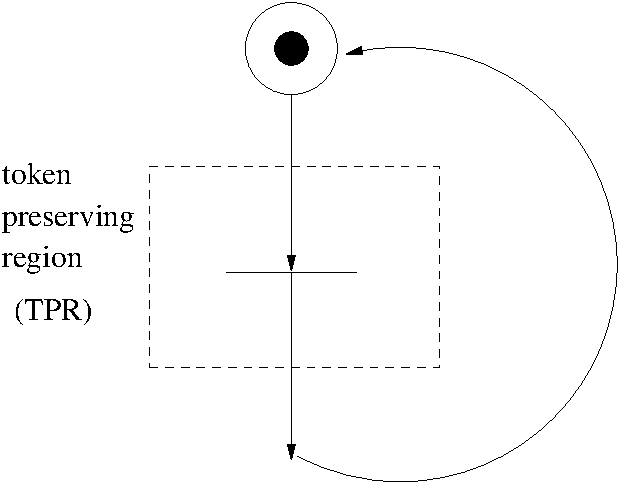
\includegraphics[width=8cm]{figs/BaseCP.pdf}
  \caption{Starting point: control Petri-net}
\end{figure}
}

\frame[containsverbatim]{\frametitle{Series augmentation}
\begin{figure}
  \centering
  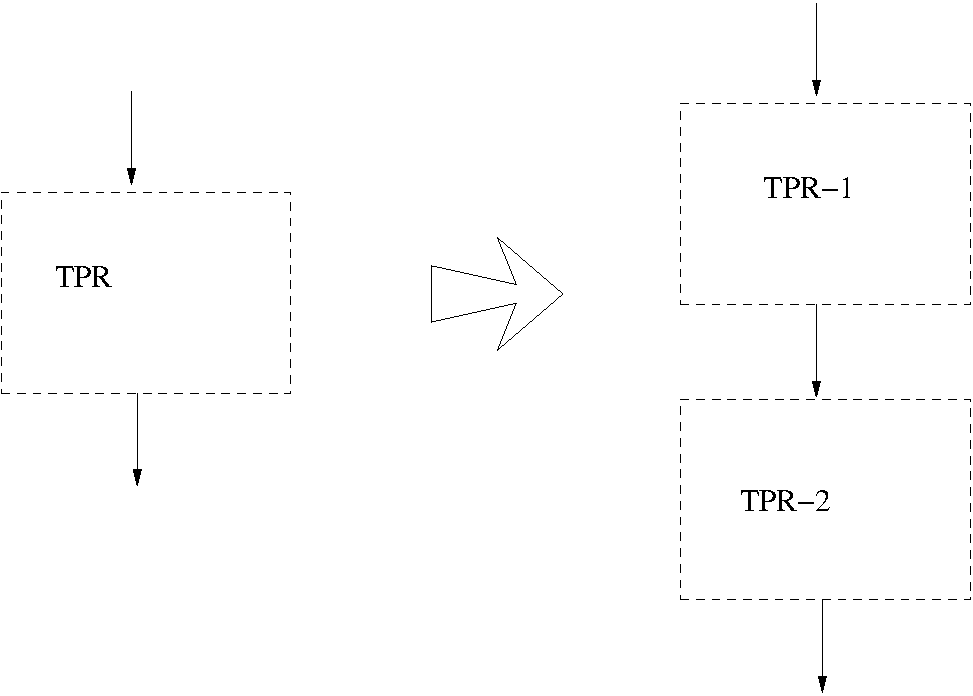
\includegraphics[width=10cm]{figs/SeriesCP.pdf}
  \caption{Series augmentation}
\end{figure}
}

\frame[containsverbatim]{\frametitle{Parallel augmentation}
\begin{figure}
  \centering
  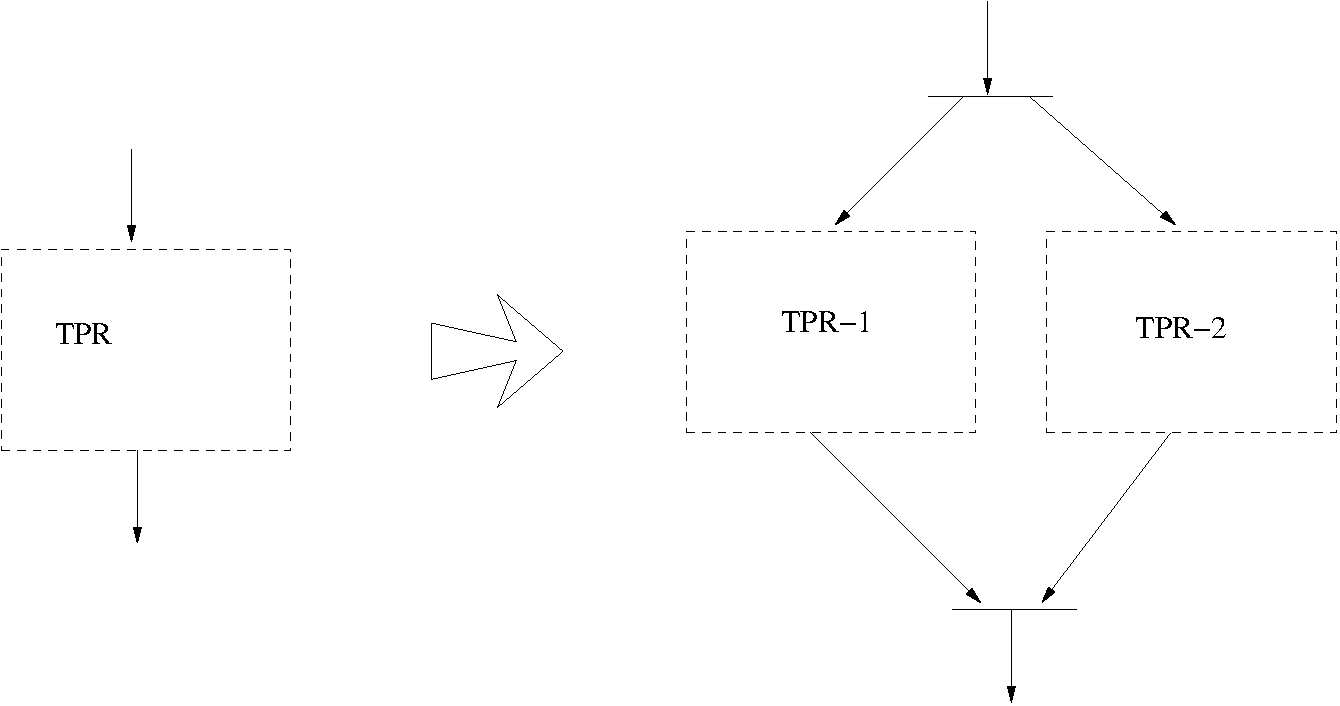
\includegraphics[width=10cm]{figs/ParallelCP.pdf}
  \caption{Series augmentation}
\end{figure}
}

\frame[containsverbatim]{\frametitle{Branch augmentation}
\begin{figure}
  \centering
  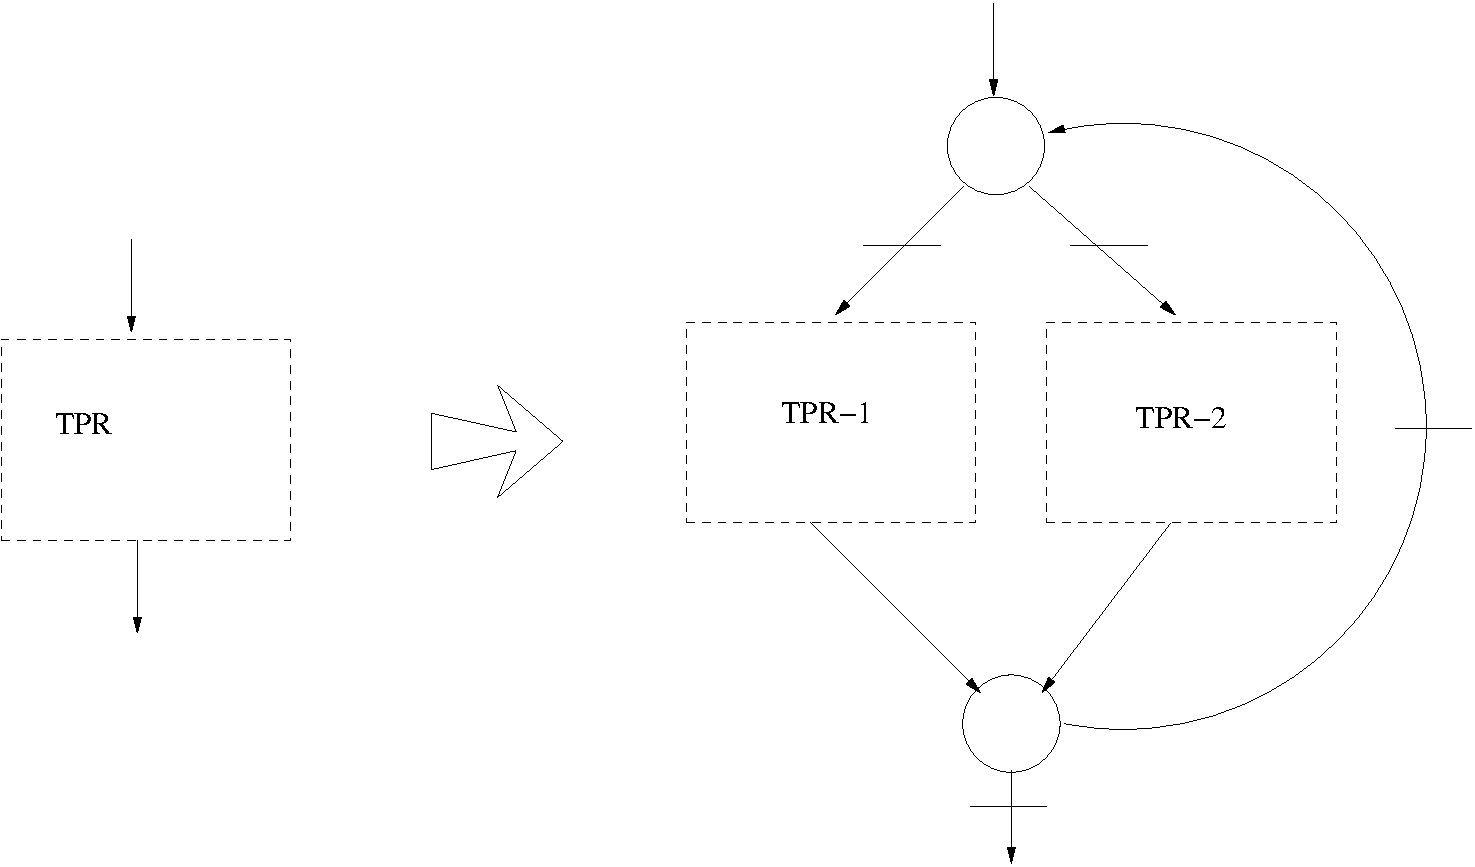
\includegraphics[width=10cm]{figs/BranchCP.pdf}
  \caption{Branch augmentation}
\end{figure}
}

\frame[containsverbatim]{\frametitle{Fork augmentation}
\begin{figure}
  \centering
  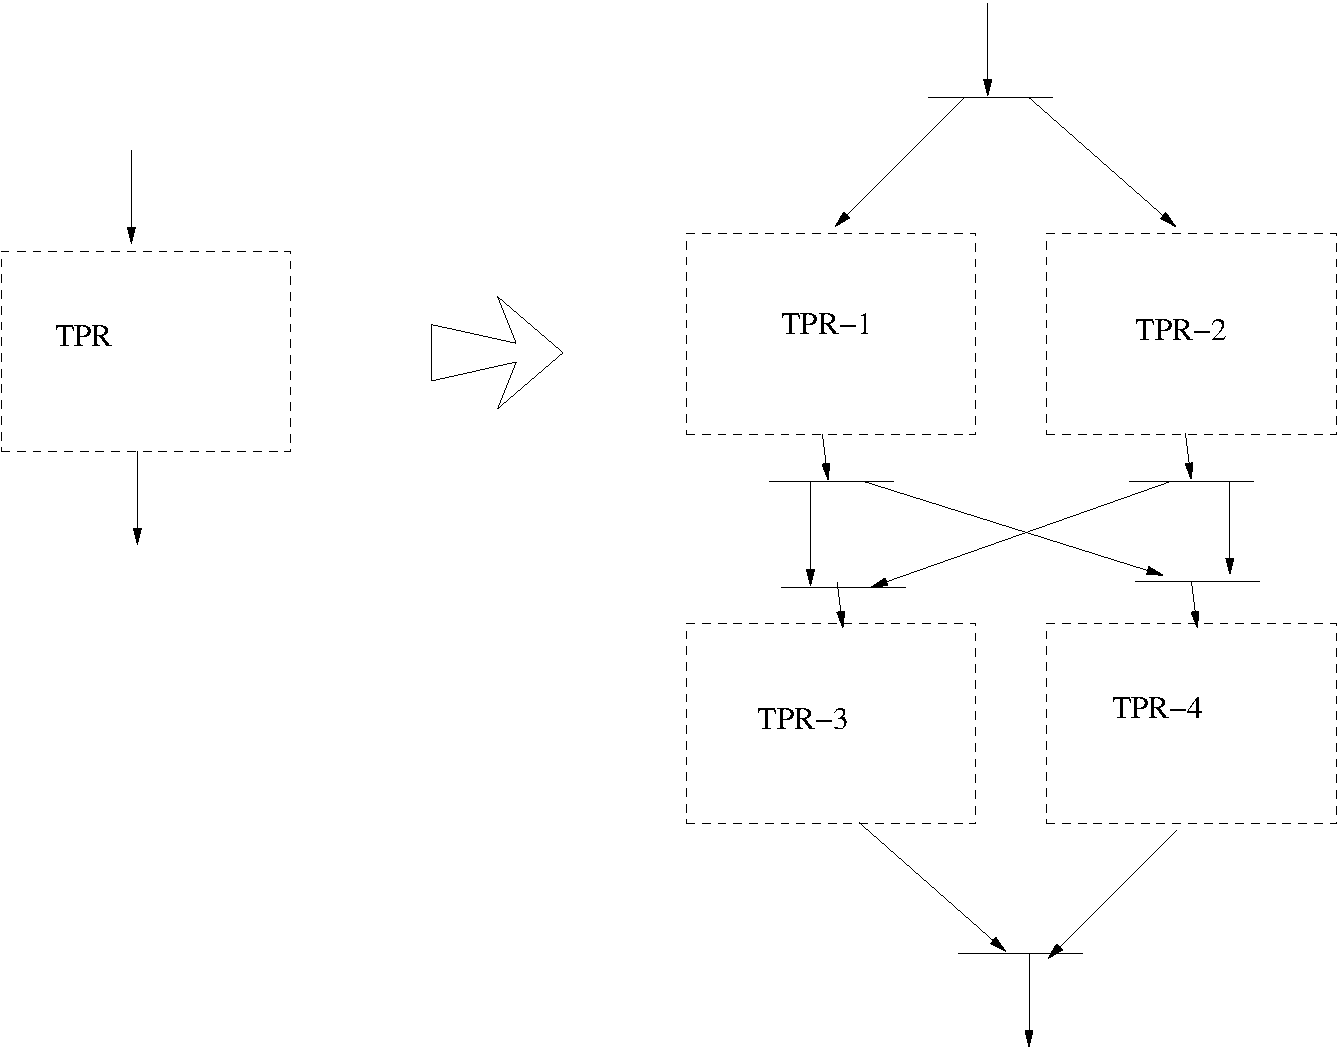
\includegraphics[width=10cm]{figs/ForkCP.pdf}
  \caption{Fork augmentation}
\end{figure}
}

\frame[containsverbatim]{\frametitle{Implementation of control net}
\begin{figure}
  \centering
  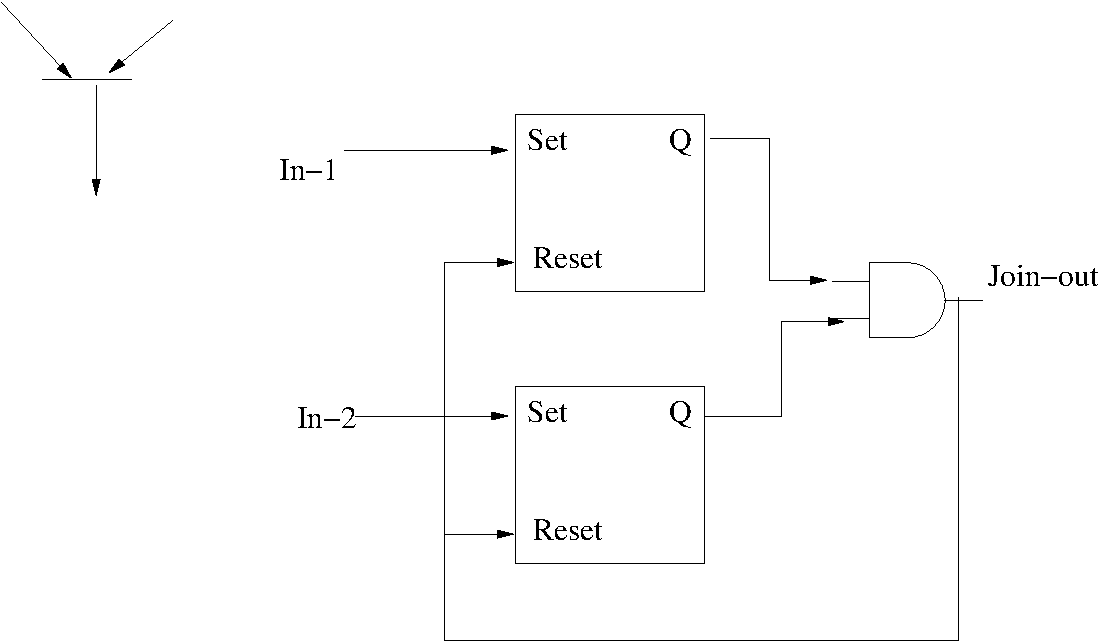
\includegraphics[width=10cm]{figs/Join.pdf}
  \caption{Two-input join logic implementation}
\end{figure}
}

\frame[containsverbatim]{\frametitle{The control path:  a summary}
\begin{itemize}
\item Constructed as a Petri-net by following certain rules.
\begin{itemize}
\item The resultant Petri-net is safe (and hence can be implemented
as a logic circuit).
\end{itemize}
\item Implementation of the control path using logic gates is easy.
\begin{itemize}
\item Only join transitions need actual logic gates.
\end{itemize}
\item  Sufficient to model control-flow in most high level programming
languages.
\end{itemize}
}

\frame[containsverbatim]{\frametitle{Other constituents of the AHIR hardware}
\begin{itemize}
\item Pipes:  FIFO with multiple writers and readers.
\item Memory sub-systems: first initiated first served guarantee.
\item Multiplexors: with tagged and untagged functionality.
\item Arbiters: fair arbitration (round-robin).
\end{itemize}
}

\frame[containsverbatim]{\frametitle{Pipes}
\begin{figure}
  \centering
  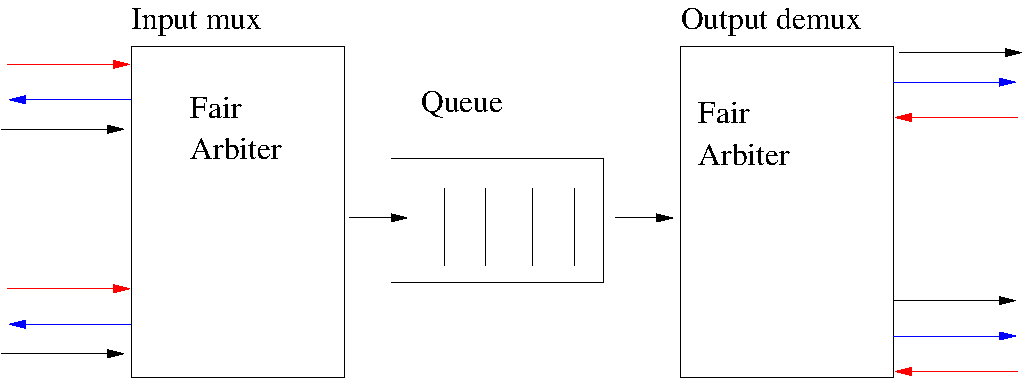
\includegraphics[width=10cm]{figs/Pipe.pdf}
  \caption{Pipes}
\end{figure}
}

\frame[containsverbatim]{\frametitle{Memory sub-system}
\begin{figure}
  \centering
  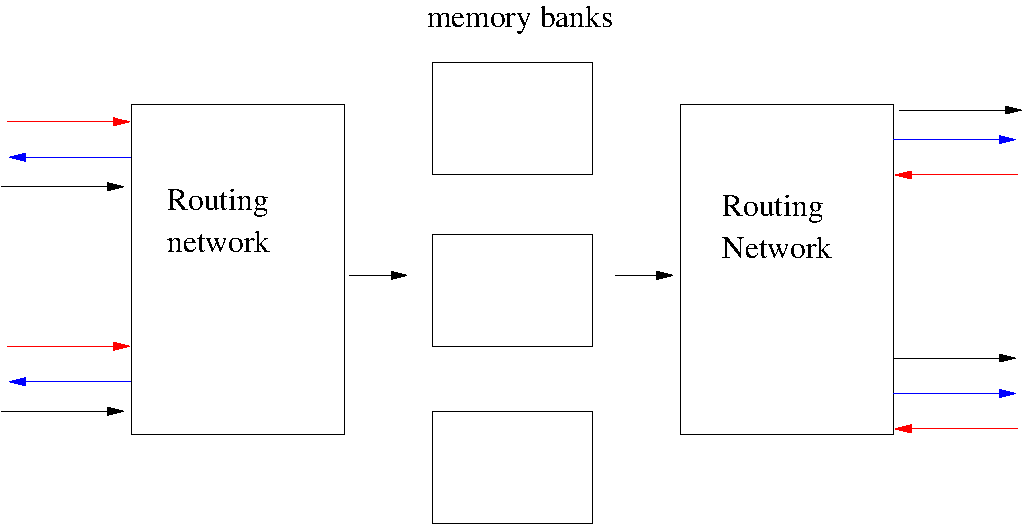
\includegraphics[width=10cm]{figs/MemorySubsystem.pdf}
  \caption{Memory sub-system}
\end{figure}
}

\frame[containsverbatim]{\frametitle{Lets take a look}
Go back to earlier example of FIR filter and check it out.
}
\end{document}
